En esta sección, vamos a comprobar empíricamente que nuestro algoritmo tiene una complejidad temporal cúbica respecto de n, y lineal respecto de k.

En un primer caso, utilizamos instancias donde cada casillero tiene una potencia en función de n: p(n) = $n/5$. Una vez más, utilizamos k distintos entre sí, pero fijos en cada caso. Probamos con distintos $n$ y obtuvimos el resultado que se puede observar en las figuras debajo.

\begin{figure}[H]
  \begin{minipage}{0.5\linewidth}
    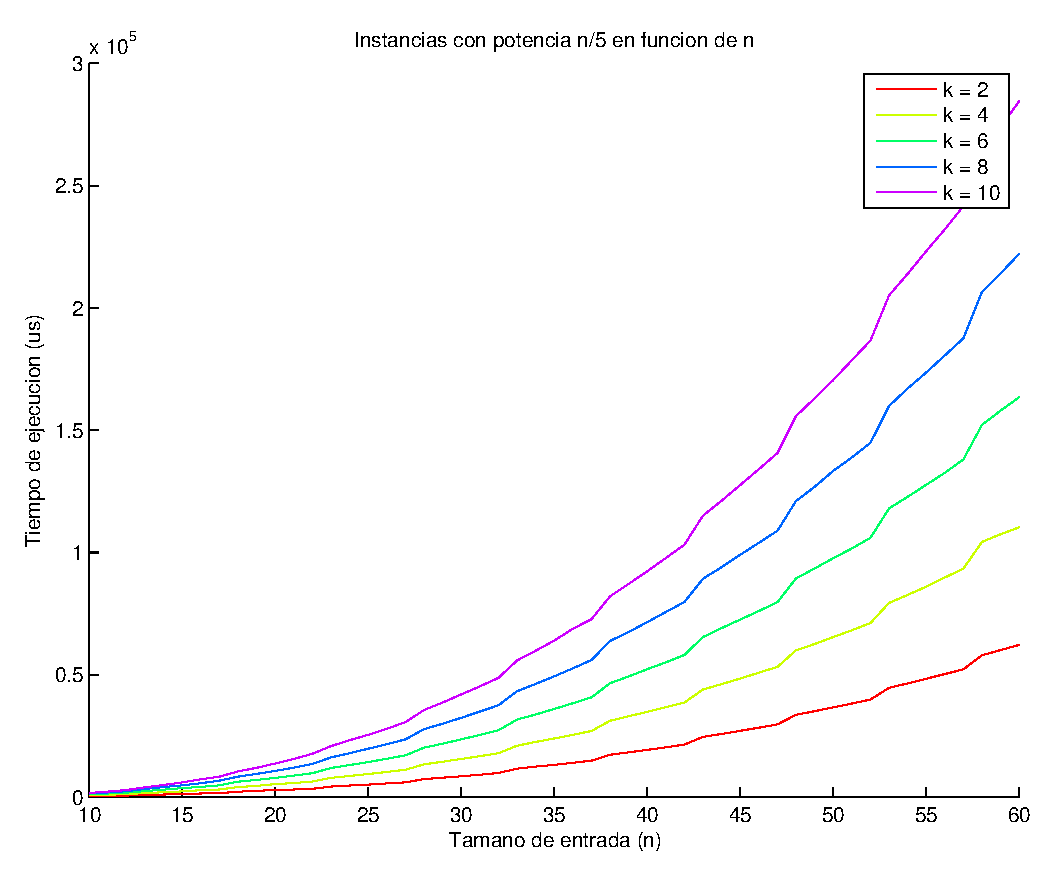
\includegraphics[width=\linewidth]{img/problema3/instancia_p_20p_varios_k.eps}
    \caption{Tiempo de ejecución, p(n) = $n/5$}\label{fig:problema3-k-20}
  \end{minipage}
  \hfill
  \begin{minipage}{0.5\linewidth}
    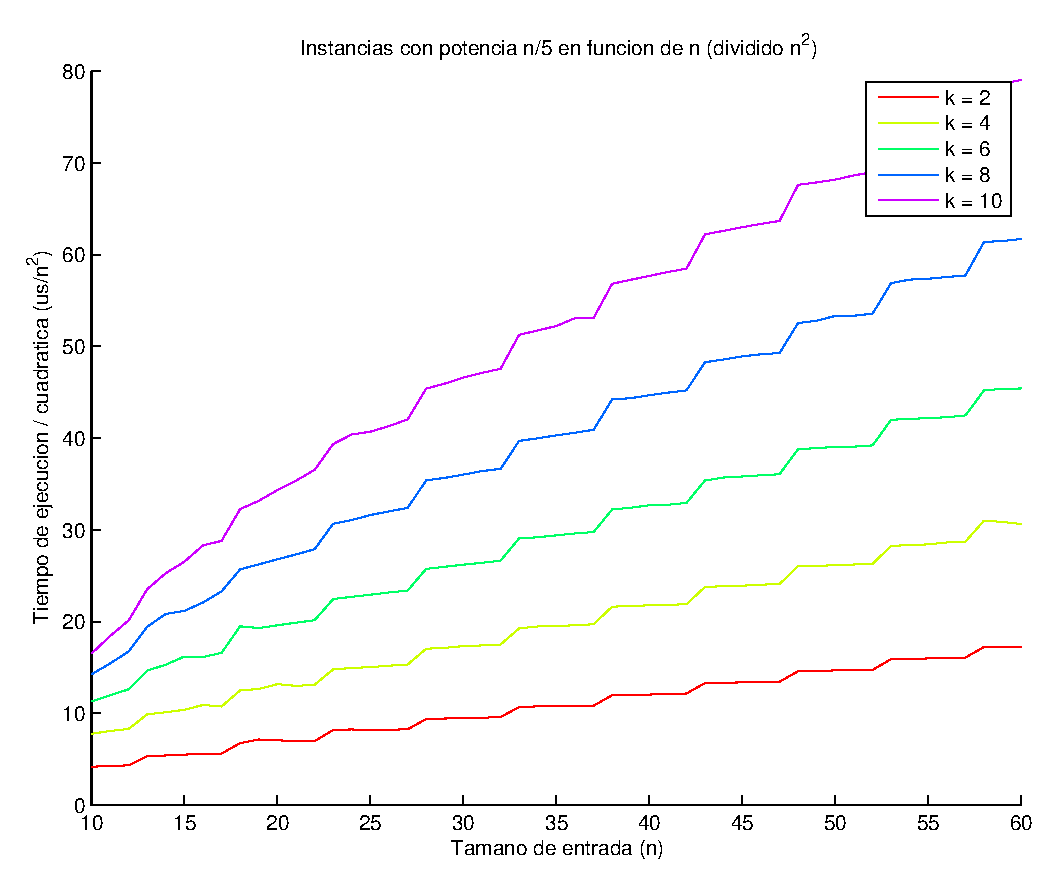
\includegraphics[width=\linewidth]{img/problema3/instancia_p_20p_varios_k_div_n2.eps}
    \caption{Idem, dividido por $n^2$}\label{fig:problema3-k-n2-20}
  \end{minipage}	
\end{figure}

En la figura \ref{fig:problema3-k-20} no podemos notar la complejidad temporal de la función. Por esto, dividimos por $n^2$ y plasmamos ese resultado en la figura \ref{fig:problema3-k-n2-20}. Sin embargo, en esta última figura tampoco podemos ver claramente la complejidad temporal. Por esta razón, decidimos analizar los ``saltos'' que se ven en $T(n)$. Luego de experimentación y búsqueda llegamos a la conclusión que esos saltos se relacionan con el cambio de potencia de los resortes. Por ejemplo entre para n entre 10 y 15 las potencias son de la siguiente manera: 2,2,2,3,3,3 respectivamente. Esto se debe a que 12/5 = 2.4 (y lo redondea para abajo) y 13/5 = 2.6 (que se redondea para arriba) por lo tanto entre n = 12 y n = 15 va a haber un salto.

Una vez que entendimos estos saltos, llegamos a la conclusión que si tomamos los puntos donde éstos se encuentran en la función y trazamos una recta $r$, la recta correspondiente al tiempo de ejecución va a tener una pendiente menor o igual a la pendiente de la recta $r$. Es decir, que comprobamos que por más que la potencia dependa del n la complejidad temporal también es lineal respecto de $T(N)/n^2$ que es lo mismo que decir que es cúbica respecto de n.

Finalmente, decidimos hacer un experimento más: utilizamos n distintos entre sí (pero fijos en cada caso) y variar el k. Una vez más p depende de n con la misma función anteriormente usada.

\begin{figure}[H]
  \begin{minipage}{0.5\linewidth}
    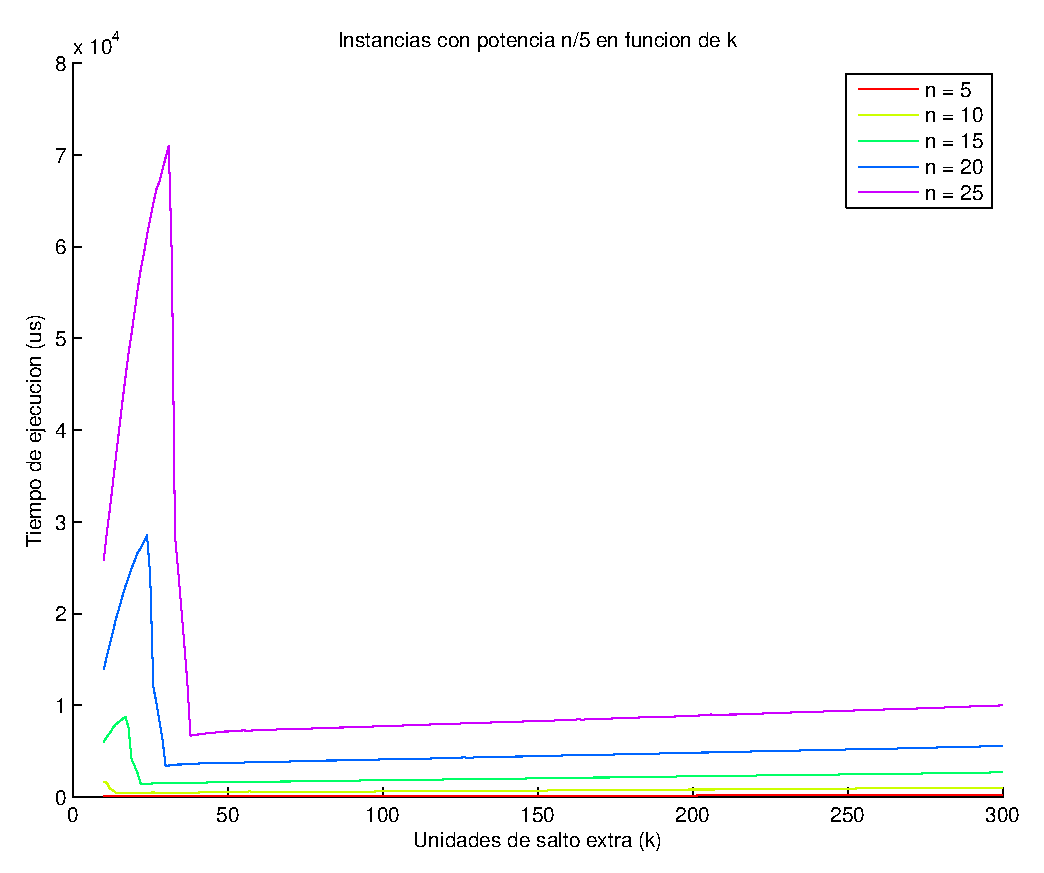
\includegraphics[width=\linewidth]{img/problema3/instancia_p_20p_varios_n.eps}
    \caption{Tiempo de ejecución, p(n) = $n/5$}\label{fig:problema3-n-20}
  \end{minipage}
  \hfill
  \begin{minipage}{0.5\linewidth}
    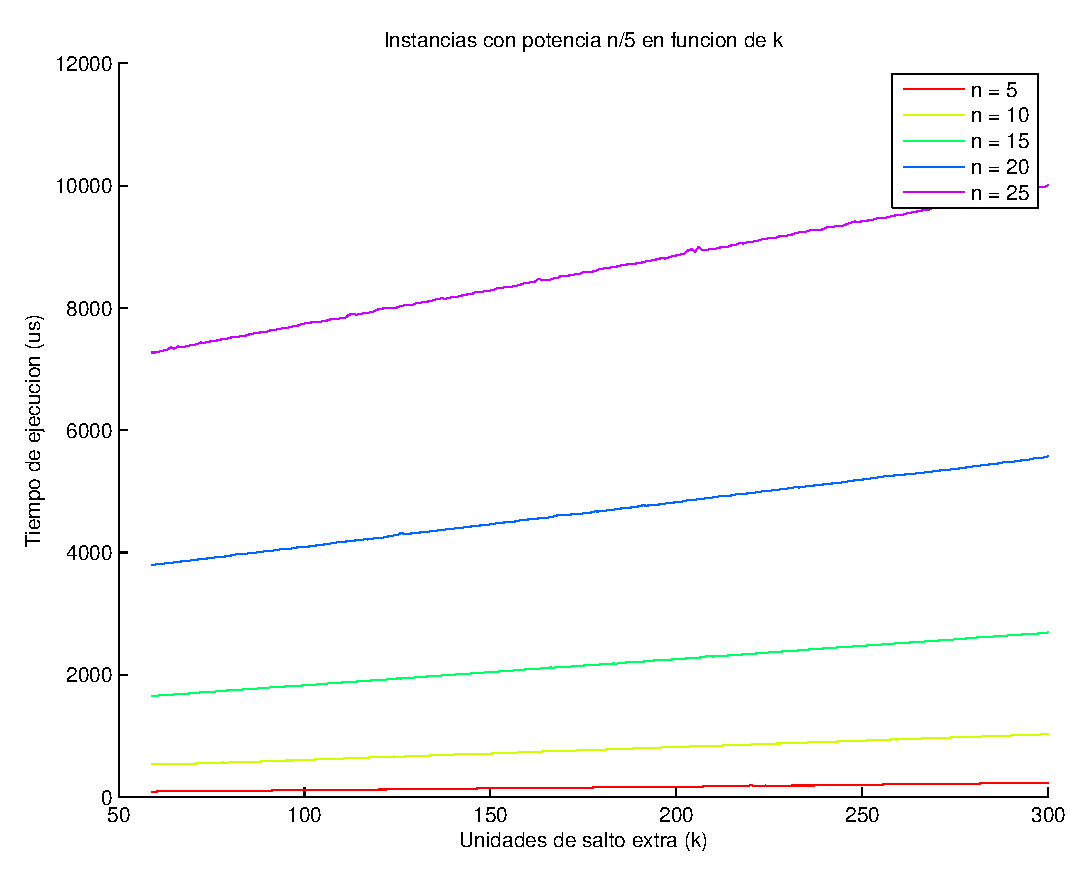
\includegraphics[width=\linewidth]{img/problema3/instancia_p_20p_varios_n_zoom.eps}
    \caption{Idem, con \emph{zoom}}\label{fig:problema3-n-n2-20}
  \end{minipage}
\end{figure}

En estos casos, una vez más podemos observar que cuando $k \geq 2*(n-1-p)$ resolver el problema es trivial. En estas figuras, está representado por la caída del tiempo de ejecución a partir de este punto. Cabe aclarar que si bien resolver el problema es trivial, al crecer el n cuesta más crear la matriz3D ya que la misma es más grande. En estos casos, la complejidad temporal de nuestro algoritmo es lineal respecto de k.

Para poder ver mejor esto último, realizamos \emph{zoom} a la figura a partir del momento de la caída, lo cual lo podemos ver en la figura \ref{fig:problema3-n-n2-20}. En esta figura, se ve claramente que la complejidad temporal de nuestro algoritmo es lineal respecto de k.

%TODO les parece poner un apendice con mas graficos o lo dejamos asi?